


\chapter{Grundlagen}\label{basics}
\section{Fazialisparese}\label{facialpalsy}
Fazialisparese (eng. Facial nerve Paralysis) ist eine Funktiosstörung der Hirnnerven und der mimischen Gesichtsmuskulatur. Durch diese Nervenbahnstörung können eine partielle oder auch vollständige Beeinträchtigung der Muskeln im Gesicht ausgeprägt sein. Dabei werden vor allem der Lidschluss, Strinbewegungen (runzeln und Augenbraun heben), Mundwinkel und Lippenschluss als offensichtliche Merkmale negativ beeinflusst. Auch können Geschmack, Hörsinn, Speichel und Tränenfluss in Mitleidenschaft gezogen sein \cite{facialpalsy_1}\cite{facialpalsy_2}.

Liste von Ursachen für die Ausprägung einer Fazialisparese:
\begin{itemize}
  \setlength\itemsep{-0.5em}
\item Infektionen (z.B. Borrelien)
\item Entzündungen
\item Traumatische oder geburtstraumatische
Schädigung
\item Tumore
\item Angeborener Defekt
\item Idiopathisch (Bell-Parese)
\item Verletzung des Nerves
\end{itemize}




\paragraph{House-Brackmann Skala} ist ein Score der für die Ermittlung des Schweregrades der Fazialisparese Anwendung findet. Das Sytsem beinhaltet eine 6-Punkte Skala von \textbf{I} normal bis \textbf{IV} vollständig ausgeprägte Parese (Tabelle \ref{cap:housebrackmann}) \cite{housebrackmann}.

\textbf{TODO}

\vspace{7cm}

\begin{table}[!tb]\vspace{1ex}\centering
  \resizebox{0.85\textwidth}{!}{
  \small
  \begin{tabular*}{15.5cm}{c||c|cccc|}
%\hline
\multirow{2}{*}{\textbf{Grad}} &
  \multirow{2}{*}{\textbf{Beschreibung}} &
  \multicolumn{1}{c|}{\textbf{Statisch}} &
  \multicolumn{3}{c|}{\textbf{Dynamisch}} \\ \cline{3-6}
 &
   &
  \multicolumn{1}{c|}{\textbf{Symmetrie}} &
  \multicolumn{1}{c|}{\textbf{Stirn}} &
  \multicolumn{1}{c|}{\textbf{Lidschluss}} &
  \textbf{Mund} \\ \hline\hline
I &
  Normal &
  \multicolumn{4}{c|}{Normal} \\ \hline
II &
  \begin{tabular}[c]{@{}c@{}}Leichte\\ Funktionsstörung\end{tabular} &
  \multicolumn{1}{c|}{Normal} &
  \multicolumn{1}{c|}{\begin{tabular}[c]{@{}c@{}}moderate\\ bis\\ gute\\ Funktion\end{tabular}} &
  \multicolumn{1}{c|}{\begin{tabular}[c]{@{}c@{}}geschlossen,\\ minimale\\ Anstrengung\end{tabular}} &
  \begin{tabular}[c]{@{}c@{}}leichte\\ Asymmetrie\end{tabular} \\ \hline
III &
  \begin{tabular}[c]{@{}c@{}}Moderate\\ Funktionsstörung\end{tabular} &
  \multicolumn{1}{c|}{Normal} &
  \multicolumn{1}{c|}{\begin{tabular}[c]{@{}c@{}}leicht\\ bis\\ moderate\\ Funktion\end{tabular}} &
  \multicolumn{1}{c|}{\begin{tabular}[c]{@{}c@{}}geschlossen,\\ maximale\\ Anstrengung\end{tabular}} &
  \begin{tabular}[c]{@{}c@{}}leicht Betroffen,\\ maximale\\ Anstrengung\end{tabular} \\ \hline
IV &
  \begin{tabular}[c]{@{}c@{}}Mittelschwere\\ Funktionsstörung\end{tabular} &
  \multicolumn{1}{c|}{Normal} &
  \multicolumn{1}{c|}{keine} &
  \multicolumn{1}{c|}{unvollständig} &
  \begin{tabular}[c]{@{}c@{}}Asymmetrisch,\\ maximale\\ Anstrengung\end{tabular} \\ \hline
V &
  \begin{tabular}[c]{@{}c@{}}Schwere\\ Funktionsstörung\end{tabular} &
  \multicolumn{1}{c|}{Asymmetrisch} &
  \multicolumn{1}{c|}{keine} &
  \multicolumn{1}{c|}{unvollständig} &
  \begin{tabular}[c]{@{}c@{}}leichte\\ Bewegung\end{tabular} \\ \hline
VI &
  komplette Parese &
  \multicolumn{4}{c|}{keine} \\ \hline
  \end{tabular*}
  }
  \caption[Schweregradeinteilung der Fazialisparese nach House-Brackmann]{Schweregradeinteilung der Fazialisparese nach House-Brackmann \cite{housebrackmann}}\label{cap:housebrackmann}
\vspace{2ex}\end{table}\label{table:housebrackmann}


\section{Maschinelles Lernen und Neuronale Netze}\label{neuralnet}
\paragraph{Maschinelles Lernen} ist ein Teilgebiet der Künstlichen Intelligenz umfassd im Allgemeinen, durch Methoden und Lernporzesse Zusammenhänge in Datensätzen zu erkennen. Darauf basierend sollen Vohersagen getroffen werden. Ein Optimierungsproblem soll so gelöst werden, das aus einer Korrelation zwischen einem Ausgabewert und der Eingabe besteht. Durch selbstlernende Algroithmen sollen diese Modelle die Vorhersagegenauigkeit selber anpassen und den Ausgabewert in der Genauigkeit verbessern, ohne dabei den Algorithmus explizit zu programmieren zu müssen \cite{machinelearning_1} \cite{machinelearning_2}.

Diese  Lernverfahren können in drei Kategorien aufgeteilt werden:
\begin{itemize}
  \setlength\itemsep{-0.5em}
\item Überwachtes Lernen
\item Unbewachtes Lernen
\item Bestärkendes Lernen
\end{itemize}

Bei dem überwachten Lernverfahren wird das Modell trainiert, um ein Ausgabewert eines nicht bekannten Datensatzes (Validations-Datensatz) verhergesagt werden kann. Ziel ist die Genauuigkeit dieser Vorhersage zu maximieren. Das Gegenteil davon das unbewachte Verfahren. Dabei die Ausgabe nicht bekannt oder es kann keine präzise Aussage darüber getroffen werden. Anhand der Eingabe sollen so Muster und Zusammenhäne herausgefunden werden. Bestärkendes Lenen, beschreibt eine Methode, womit das Modelll bestraft, oder belohnt wird um ein Ergebnis zu optimieren \cite{machinelearning_1}.

Im Verlauf dieser Arbeit wird nur das \textbf{überwachte Lernen} der Modelle betrachtet.


\paragraph{Neuronale Netze} werden vor allem für die Klassifikation von Daten und Regression eingesetzt. Hierbei werden Parameter des Netzes optimeirt, die zwischen den einzelnen Schichten (eng. Layer) liegen. Nicht-Lineare Aktivierungsfunktionen transformieren Eingabewerte in andersliegende Wertebereiche. Ergebnisse dieser Funktion dienen in weiterführende Schichten als Eingabe (Abb. \ref{cap:neuralnet}). Diese Layer können auch eine diskrete Faltung oder eine Normalisierung dieser darstellen. In Kombination mit der Verschachtelung der verschiedensten Layer können so belibig komplizierte Modelle gebildet werden \cite{machinelearning_3}.


\def\layersep{2.5cm}
\begin{figure}[!tb]
\begin{center}
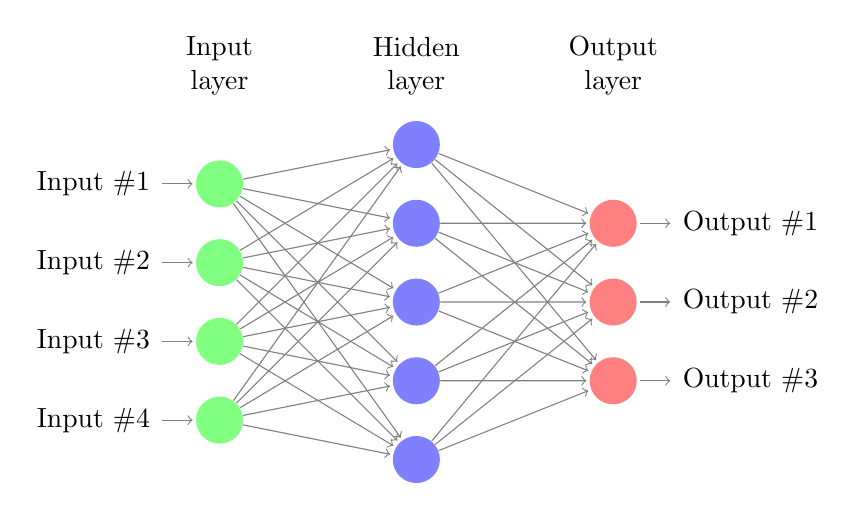
\begin{tikzpicture}[shorten >=1pt,->,draw=black!50, node distance=\layersep]
    \tikzstyle{every pin edge}=[<-,shorten <=1pt]
    \tikzstyle{neuron}=[circle,fill=black!25,minimum size=17pt,inner sep=0pt]
    \tikzstyle{input neuron}=[neuron, fill=green!50];
    \tikzstyle{output neuron}=[neuron, fill=red!50];
    \tikzstyle{hidden neuron}=[neuron, fill=blue!50];
    \tikzstyle{annot} = [text width=4em, text centered]

    % Draw the input layer nodes
    \foreach \name in {1,...,4}
        \node[input neuron, pin=left:Input \#\name] (I-\name) at (0,-\name) {};

    % Draw the hidden layer nodes
    \foreach \name in {1,...,5}
        \path[yshift=0.5cm]
            node[hidden neuron] (H-\name) at (\layersep,-\name cm) {};

    % Draw the input layer nodes
    \foreach \name in {1,...,3}
      \node[output neuron, pin={[pin edge={->}]right:Output \#\name}] (O-\name) at (2*\layersep,-0.5cm-\name cm) {};

    % Connect every node in the input layer with the hidden layer.
    \foreach \source in {1,...,4}
        \foreach \dest in {1,...,5}
            \path (I-\source) edge (H-\dest);

    % Connect every node in the hidden layer with the output layer
    \foreach \source in {1,...,5}
        \foreach \dest in {1,...,3}
            \path (H-\source) edge (O-\dest);

    % Annotate the layers
    \node[annot,above of=H-1, node distance=1cm] (hl) {Hidden layer};
    \node[annot,left of=hl] {Input layer};
    \node[annot,right of=hl] {Output layer};
\end{tikzpicture}
\caption[Beispielaufbau eines Neuronale Netzes]{Beispielaufbau eines Neuronale Netzes. Die Input Layer repräsentieren die Eingabe in das Netz. Hidden Layer sind versteckte Schichten im Modell. Die Ausgabe auf der linken Seite sind bei einer Klassifikation Wahrscheinlichkeiten, bezogen auf die  zu erwartenden Label. Die Kanten zwischen den Schichten haben Gewichte ahand deren die Eingabe modifiziert wird.}\label{cap:neuralnet}
\end{center}
\end{figure}\label{fig:neuralnet}

Das Training dieser Netze basiert auf Forwärts- und Rückwärtsrechnen dier Geichte und Parameter an den Kanten. Dabei läuft zuerst die Eingabe des neuronalen Netzes alle Schichten, die eine Reihe von Transformationen ausführt. Das Ergebnis nach den Durchlauf wird mit dem realen Ergebnis verglichen, das innerhalb der Trainingsphase bekannt ist. Die Abweichung von diesem Vergleich, auck bekannt als Fehler, wird in der umgekehrten Richtung durch das Netzwerk geschickt. Die Gewichte an den Kanten zwischen den Layern werden anhand des Fehlers angepasst. So soll erreicht werden, dass das Netz sich im Verhalten der Ein- und Ausgabe konvergiert.

%\clearpage
\section{Gesichtserkennung}\label{facedetection}
\textbf{TODO}

\section{Automatentheorie}\label{automatatheory}
\textbf{TODO}





\chapter{Stand der Technik}\label{std}

Im Folgenden Kapitel soll der momentane  Stand der Technik für die zugrunge liegende Aufgabenstellung erläutert werden. Der Abschnitt \ref{segmentation} veranschaulicht dabei die Graduierung der Fazialisparese mithilfe von Segmentierung basierte Methoden.
\textbf{TODO}

\section{Segmentierung basierte Methoden}\label{segmentation}
\textbf{TODO}


\paragraph{Deep-Learning basierte semantische Segmentierung zur Extraktion von Gesichtsattributen}
TMP \cite{detection_fp2}.

\textbf{TODO}
